\documentclass[spanish]{beamer}
\usepackage[ansinew]{inputenc} % Acepta caracteres en castellano
\usepackage[spanish]{babel}    % silabea palabras castellanas
\usepackage{amsmath}
\usepackage{mathtools,cancel} % cancela con una flecha \cancelto{0}{XXXX}
\renewcommand{\CancelColor}{\color{red}} %change cancel color to red
\usepackage{amsfonts}
\usepackage{amssymb}
\usepackage{dsfont}
\usepackage{graphicx}
\usepackage{geometry}
\usetheme{Madrid}
\usecolortheme{beaver}
\usepackage{textpos}
% Logo  en el comienzo 
\addtobeamertemplate{frametitle}{}{%
\begin{textblock*}{100mm}(.85\textwidth,-1cm)
{\includegraphics[height=0.4in, keepaspectratio=true]{/Users/luisnunez/Dropbox/MisDocumentos/UIS/UISImagenInstitucional/UISLOGO.png}}
\end{textblock*}}

\begin{document}

\title{\textbf{Potencial efectivo} }
\author[L.A. N��ez]{\textbf{Luis A. N��ez}}  
\institute[UIS]{\textit{Escuela de F�sica, Facultad de Ciencias, } \\
\textit{Universidad Industrial de Santander, Santander, Colombia } \\
{\includegraphics[height=0.4in, keepaspectratio=true]{/Users/luisnunez/Dropbox/MisDocumentos/UIS/UISImagenInstitucional/UISLOGO.png}}
}
\date{\today}
\maketitle


\begin{frame}
\frametitle{Agenda}
  \tableofcontents
\end{frame}


%%%%% Diapo 1
\section{El potencial efectivo}
\frame{
  \frametitle{El potencial efectivo}
   \begin{itemize}  
  	\item<1-> Para el problema de dos cuerpos con un potencial central $V(r)$ 
	$\mathcal{L}=\frac{1}{2} \mu\left(\dot{r}^2+r^2 \dot{\theta^2}\right)-V(r) \Rightarrow \frac{d}{d t}\left(\frac{\partial \mathcal{L}}{\partial \dot{r}}\right)-\frac{\partial \mathcal{L}}{\partial r}=0 \Rightarrow \mu \ddot{r}=-\frac{\partial V}{\partial r}+\frac{L^2}{\mu r^3}$
	\item<2-> La fuerza radial $f(r)=-\frac{\partial V}{\partial r}$ entonces $\mu \ddot{r}=f(r)+\frac{L^2}{\mu r^3} \Rightarrow \mu \ddot{r}=f_{\mathrm{ef}}(r)$
	\item<3-> La fuerza efectiva surge de las contribuciones de la fuerza central $f(r)=-\frac{\partial V}{\partial r}$ y el efecto no inercial $F_{ni} \equiv \frac{L^2}{\mu r^3}=\mu r \dot{\theta}^2$
	\item<4-> Se define una energ�a potencial efectiva, $V_{\mathrm{ef}}(r) \equiv V(r)+\frac{L^2}{2 \mu r^2}$,  tal que $f_{\mathrm{ef}}(r) \equiv-\frac{\partial V_{\mathrm{ef}}}{\partial r}$
	\item<5-> La energ�a total ser� $E  =\frac{1}{2} \mu \dot{r}^2+\frac{L^2}{2 \mu r^2}+V(r)  =\frac{1}{2} \mu \dot{r}^2+V_{\mathrm{ef}}(r)=$ cte.
	\item<6-> Una part�cula de masa $\mu$, movi�ndose en la dimensi�n $r$ con energ�a potencial $V_{\mathrm{ef}}(r)$.
    \end{itemize}
}
%%%%% Diapo 2
\section{Las trayectorias}
\frame{
  \frametitle{Las trayectorias 1/2}
   \begin{itemize}  
  	\item<1-> La condici�n $\dot{r}^2 \geq 0$ implica que este movimento ocurre para valores de $r$ tales que $E \geq V_{\mathrm{ef}}(r)$ 
	\item<2-> Los puntos de retorno est�n dados por la condici�n $\dot{r}=0$, i.e. 
	$E  =V_{\mathrm{ef}}(r)=\frac{L^2}{2 \mu r^2}+V(r)  \Rightarrow E r^2-V(r) r^2-\frac{L^2}{2 \mu}=0$
	\item<3-> Es una ecuaci�n algebraica de segundo grado en $r$ y pueden existir dos ra�ces reales, $r=r_{\min }, r=r_{\max }$. 
	\begin{figure}[t]
		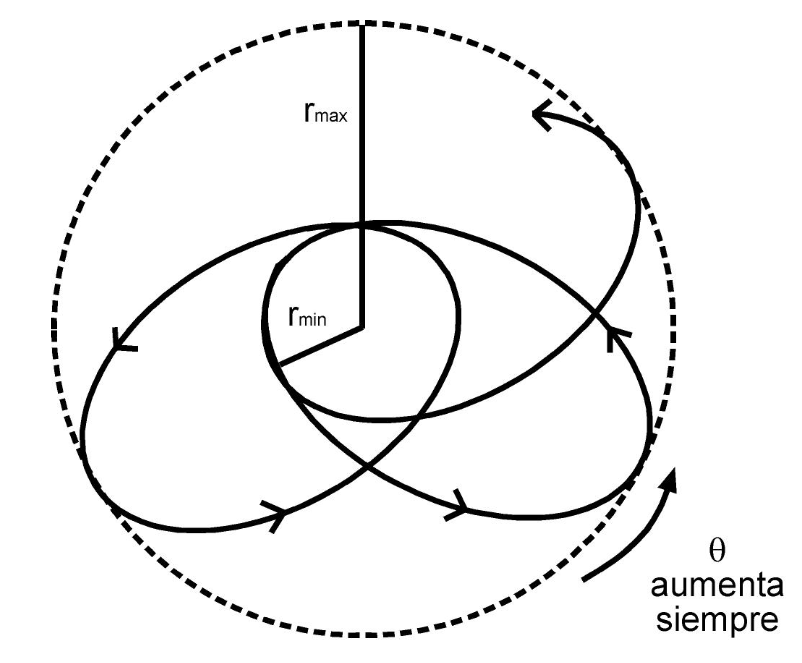
\includegraphics[width=1.5in]{Figuras/Trayectorias.png}
   	\end{figure}
	\begin{itemize}
		\item si $\quad r_{\max }<\infty \quad \Rightarrow$ movimiento es finito, oscilatorio en $r$,
		\item si $\quad r_{\max } \rightarrow \infty \quad \Rightarrow$ movimiento sin retorno,
		\item si $\quad r_{\min }=r_{\max } \quad \Rightarrow$ movimiento es circular.
	\end{itemize}

    \end{itemize}
}
%
% \section{Recapitulando}
\frame{
  \frametitle{Las trayectorias 2/2}
  \begin{enumerate}
	\item<1-> Como $\dot{\theta}=\frac{L}{\mu r^2} \geq 0$, la velocidad angular $\dot{\theta}$ nunca cambia de signo.
	\item<2-> El �ngulo $\theta$ siempre se incrementa en el tiempo y el movimiento siempre ocurre en una misma direcci�n sobre el plano $(r, \theta)$.
	\item<3-> Para encontrar la condici�n de choque $r \rightarrow 0$, i.e. $r_{\min }=0$
	\item<4-> De la ecuaci�n para la energ�a tenemos  
	$\frac{1}{2} \mu \dot{r}^2  =E-V(r)-\frac{L^2}{2 \mu r^2}>0  \Rightarrow E r^2-V(r) r^2-\frac{L^2}{2 \mu}>0$
	\item<5-> Tomando el l�mite $r \rightarrow 0$ tendremos $\lim _{r \rightarrow 0}\left[V(r) r^2\right]<-\frac{L^2}{2 \mu}$
	\item<6-> Consideremos un potencial atractivo de la forma $V(r)=-k / r^n$, entonces $\lim _{r \rightarrow 0}\left[V(r) r^2\right]<-\frac{L^2}{2 \mu} \Rightarrow n>2$
	\begin{itemize}
		\item $V(r)=-k / r^3$ permite caer al centro, $r_{\min }=0$
		\item $V(r)=-k / r^2$, requiere $k>\frac{L^2}{2 \mu}$ para caer al centro de atracci�n
		\item $V(r)=-k / r$ no permite alcanzar $r_{\min }=0$
	\end{itemize} 
  \end{enumerate}
}
%%%%% Diapo 2
\section{Ejemplos}
\subsection{Potencial $V=-\frac{k}{r^3}$}
\frame{
  \frametitle{Potencial $V=-\frac{k}{r^3}$}
   \begin{itemize}  
  	\item<1-> Si el Potencial $V=-\frac{k}{r^3}$ el potencial efectivo ser� $V_{\mathrm{ef}}(r)=-\frac{k}{r^3}+\frac{L^2}{2 \mu r^2}$
	\begin{figure}[t]
		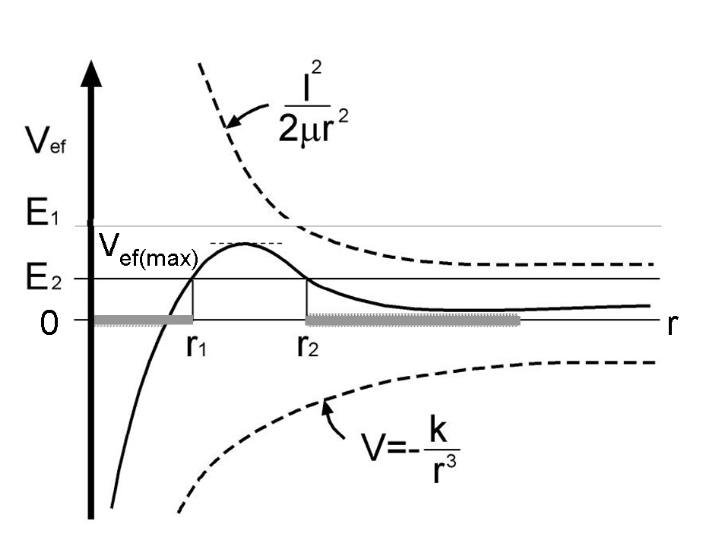
\includegraphics[width=2.0in]{Figuras/Potencialkr3.png}
   	\end{figure}
	\item<2-> El potencial efectivo exhibe un m�ximo $V_{\text {ef }(\max )}$ que representa una barrera de potencial si $E<V_{\text {ef }(\max )}$. Los posibles movimientos son
	\begin{itemize}
		\item  $E=E_1>V_{\text {ef }(\max )}$; movimiento existe $\forall r$.
		\item $E=E_2<V_{\text {ef }(\max )}$; hay dos puntos de retorno $r_1$ y $r_2$ que satisfacen $E=V_{\text {ef }}$. El movimiento ocurre para $r \in\left[0, r_1\right]$ y para $r \geq r_2$. En Mec�nica Cl�sica, el movimiento es imposible para $r \in\left[r_1, r_2\right]$.
		\item $E<0$; movimiento ocurre para $r \in\left[0, r_1\right]$.
	\end{itemize}
\end{itemize}
}
%%%%% Diapo 2
\subsection{Potencial $V=\frac{1}{2} k r^2$}
\frame{
  \frametitle{Potencial $V=\frac{1}{2} k r^2$}
   	\begin{itemize}  
  	\item<1-> Si el Potencial $V=-\frac{k}{2 \, r^2}$, el efectivo ser� $V_{\mathrm{ef}}(r)=-\frac{k}{2 r^2}+\frac{L^2}{2 \mu r^2}$
	\begin{figure}[t]
		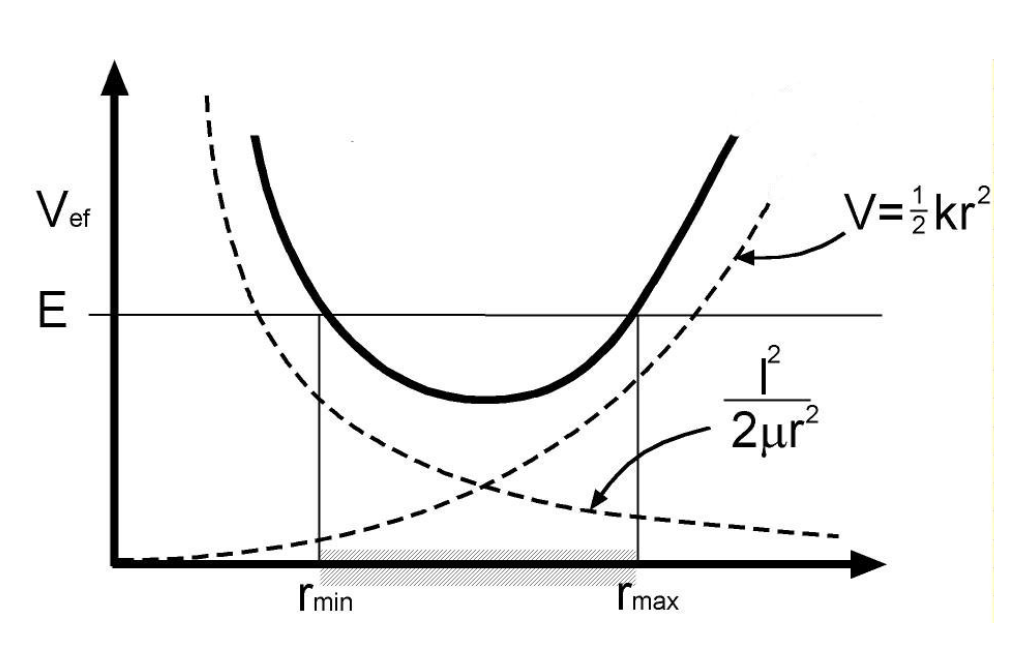
\includegraphics[width=2.0in]{Figuras/Potencialkr2.png}
   	\end{figure}
	\item<2->  $V=-\frac{k}{2 \, r^2}$ corresponde a un oscilador arm�nico tridimensional.
	\item<3->  $E \geq V_{\text {ef }}(r)$ implica que existen puntos de retorno $r_{\min }, r_{\max } \neq 0$; 
	\item<4-> Es un movimiento radial es oscilatorio.
	\item<5-> La fuerza radial $\mathbf{f}=-\frac{\partial V}{\partial r}\hat{\mathbf{r}} = -k r\hat{\mathbf{r}} = -k x {\bf i} -k y {\bf j}$ 
	\item<6-> El movimiento radial es el resultado de dos oscilaciones simples, perpendiculares entre s�, con igual frecuencia $\omega_x^2=\omega_y^2=k / \mu$.
    \end{itemize}
}
%%%%% Diapo 2
\subsection{Potencial $V=-\frac{k}{r}$}
\frame{
  \frametitle{Potencial $V=-\frac{k}{r}$}
   \begin{itemize}  
  	\item<1-> El potencial es $V=-\frac{k}{r}$, el efectivo $V_{\mathrm{ef}}=V(r)+\frac{L^2}{2 \mu r^2}=-\frac{k}{r}+\frac{L^2}{2 \mu r^2}$
	\begin{figure}[t]
		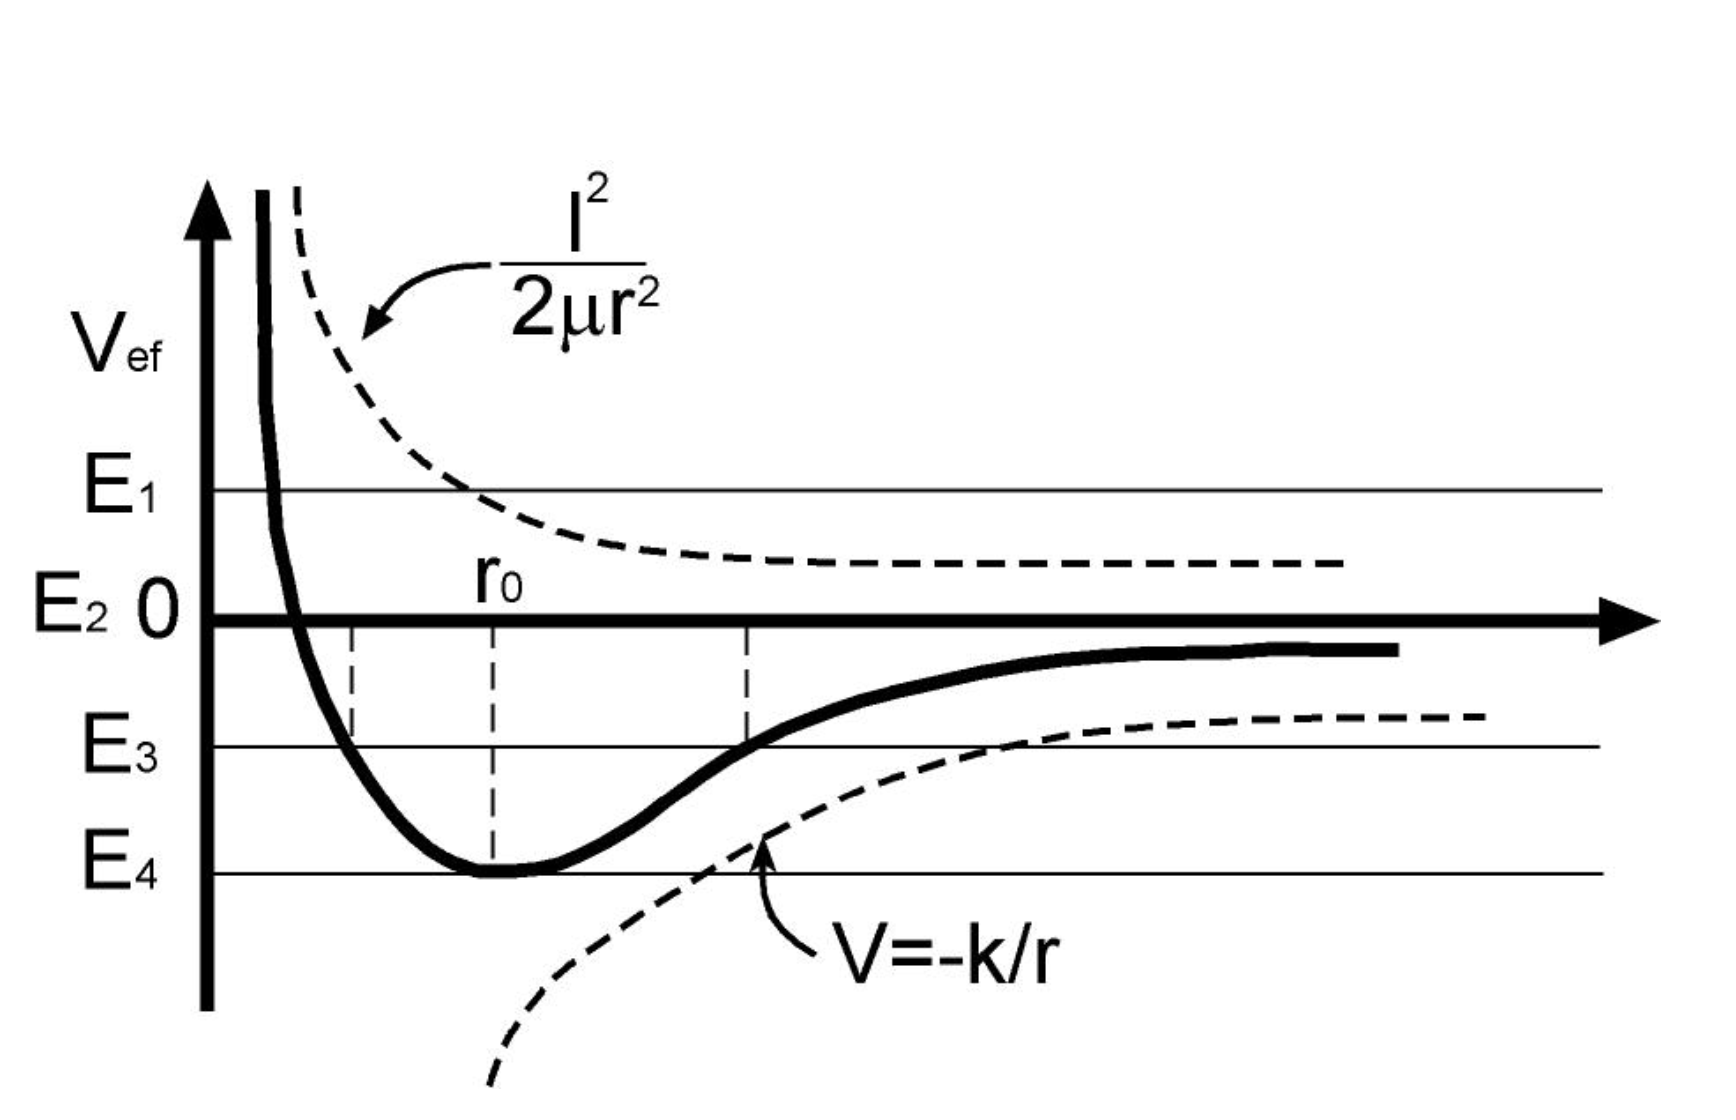
\includegraphics[width=2.0in]{Figuras/Potencialkr.png}
   	\end{figure}

	\item<2-> El valor m�nimo del potencial efectivo proviene de  $\left.\frac{\partial V_{\mathrm{ef}}}{\partial r}\right|_{r=r_0}=0$
	\item<3-> Los posibles movimientos para diferentes valores de la energ�a $E$ son:
	\begin{itemize}
		\item $E=E_1>0 \Rightarrow r_{\min }>0$ y $r_{\max } \rightarrow \infty$; �rbita abierta.
		\item $E=E_2=0 \Rightarrow r_{\min }>0$ y $r_{\max } \rightarrow \infty$; �rbita abierta.
		\item $E=E_3<0 \Rightarrow r \in\left[r_{\min }, r_{\max }\right]$; movimiento radial oscilatorio.
		\item $E=E_4=V_{\text {ef }(\min )}<0 \Rightarrow ; r_{\min }=r_{\max }=r_0$; �rbita circular con $r=r_0$.
	\end{itemize}
    \end{itemize}
}
%%%%% Diapo Recapitulando
\section{Recapitulando}
\frame{
  \frametitle{Recapitulando}
   	\begin{itemize}  
  \item<1-> 
    \end{itemize}
}
%%%%% Diapo Discusi�n
\section{Para la discusi�n}
\frame{
  \frametitle{Para la discusi�n}
   	\begin{itemize}  
  \item<1-> 
    \end{itemize}
}


  
\end{document}

%%%%% Diapo Fin
\section{Recapitulando}
\frame{
  \frametitle{Recapitulando}
En presentaci�n consideramos
  \begin{enumerate}
  	\item<1->
   \end{enumerate}
}
%%%%% Diapo 2
\section{Secci�n}
\frame{
  \frametitle{T�tulo transparencia}
   	\begin{itemize}  
  \item<1-> 
    \end{itemize}
}

